\documentclass[a4paper]{article}

\usepackage{amssymb}
\usepackage{amsmath}
\usepackage{graphicx}
\usepackage{url}
\usepackage{hhline}
\usepackage{cite}
\usepackage{tikz}
\usetikzlibrary{decorations.text}
\usepackage{ifthen}
\usepackage{booktabs}
\usepackage{placeins}
\usepackage{xcolor}
\usepackage{xspace}
\usepackage{pgfplots}
\usepackage{pgfplotstable}
\usepackage{listings}
\lstset{frame=tb,
%  language=C++,
  aboveskip=3mm,
  belowskip=3mm,
  showstringspaces=false,
  columns=flexible,
  basicstyle={\small\ttfamily},
  numbers=none,
  numberstyle=\tiny\color{gray},
  keywordstyle=\color{blue},
  commentstyle=\color{cyan},
  stringstyle=\color{green!70!black},
  breaklines=true,
  breakatwhitespace=true,
  tabsize=4,
  emph={MPI_FILE_GET_INFO,MPI_INFO_GET_NKEYS,MPI_INFO_GET_NTHKEY,MPI_INFO_GET},
  emphstyle=\color{red!75!black}
}

\newcommand{\MPIrank}{MPI rank} %% or MPI task, warnig only MPI process requires a plural -es
\newcommand{\um}[1]{_{\mathrm{#1}}}

\begin{document}

\title{KKRnano: Domain Decomposition for Efficiency}
\author{
        Paul F.~Baumeister, JSC, Forschungszentrum J{\"u}lich
%          \and
%         Marcel Bornemann, IAS-1, Forschungszentrum J{\"u}lich
%         \and
%         Rudolf Zeller, IAS-3, Forschungszentrum J{\"u}lich
        }
\date{}

\maketitle

\section{Introduction} 

KKRnano is a linear-scaling Density Functional Theory (DFT) application
optimized for the treatment of millions of atoms.
Standard DFT methods are usually limited to a few hundred atoms because of
their cubic scaling behaviour of the runtime caused by the need for matrix diagonalizations.
The KKRnano-approach is based on matrix inversion rather than diagonalizations. 
Here, direct matrix inversions are avoided and replaced by
an iterative scheme known as transpose-free quasi-minimal residual method (tfQMR).
With this and a truncation of atomic interactions beyond a certain distance
the computational complexity can be reduced to scale linearly 
with the number of atoms in the system.\cite{zeller_towards_2008,kkrnano:thiess_massively_2012}

\subsection{Short-ranged operators}

In the linear-scaling mode, a truncated view of the operator $\hat A$ 
(also called Hamiltonian due to its physical analogy)
is inverted for each source atom in the system.
$\hat A$ is a sparse operator with square-shaped blocks describing
the inter-atomic scattering.
The main computational challenge of KKRnano consists in solving
the Dyson equation (here written in terms of blocks):
\begin{equation}
 \sum_j A_{ij} \ G_{jk} = \delta_{ik}
\end{equation}
where $\delta$ is the Kronecker symbol, i.e.~block unit matrices if $i$ equals $k$.

Non-zero blocks of $\hat A$ are those connecting atomic cells that are direct neighbors in real space
(i.e.~the Voronoi cells have common faces) and, depending on the requested accuracy,
also further shells inside the so-called cluster radius $r\um{cls}$.

All blocks have the dimension $n\um{noco}(\ell\um{max} + 1)^2$
where $\ell\um{max}$ is typically $3$ and $n\um{noco}$ is $1$
for non-magentic or collinear magentic calculations 
and $2$ only for a non-collinear treatment of the spins.
Therefore, the relevant block dimensions are $16$ and $32$.

The truncation of atomic interactions $\hat G$ happens beyond a radius $r\um{trc}$
where $r\um{trc} \geq r\um{cls}$ should hold at least but is typically several times larger.
As the truncation zone is sphere-shaped around the source atom $k$, 
the set of block-rows of $\hat A$ which are relevant
for solving for the column $k$ of $\hat G$ is called its \emph{view} of $\hat A$.

\subsection{Parallelization}

The parallelization concept is to distribute the columns to different \MPIrank{}s.
In early versions, the was constrained to one atom per \MPIrank{} targetting supercomputer
architectures with a huge amount of small small compute nodes. 
In the last decade, HPC machines started to feature less nodes again 
where the performance of each node in enhanced drastically by accelerators like GPUs.

After intense code restructuring towards less \MPIrank{}s and thus several atoms per \MPIrank{}, %% Rabel, Baumeister
recent versions of KKRnano are able to make a shared usage of those block-rows of $\hat A$
that are included in the views of all columns that are treated by the same \MPIrank{}.
At first glance, the effect of sharing rows of $\hat A$ is an increased complexity
in bookkeeping. However, it comes with two striking upsides:
\begin{itemize}
 \item A reduced  memory requirement per \MPIrank{}
 \item An increased arithmentic intensity which leads to a higher percentage of the exploitable floating-point performance
\end{itemize}
The latter argument comes from the algorithmic restructuring.
The original linear solver was envoked to find the solution of 
$\hat A \ \vec x = \vec b$ with $\vec x$ being a block-vectors.
Now, we solve $\hat A \ \hat X = \hat B$ with $\hat X$ being a block-sparse matrix.
The linear solver tfQMR (transpose-free Quasi Minimal Residual method)
is an iterative scheme in which the forward multiplication $\hat A \ \hat X$
needs to be computed many times.
With the new structure, the multiplication is now closer to a matrix-matrix multiplication
than to a matrix-vector multiplication. Hence, we can exploit data re-use to effectively
save memory bandwidth. 
The overall arithmetic intensity (AI) is now higher than the base AI of the block-times-block multiplication.

\subsection{Load balancing}

In order to make the parallelization efficient,
we want to keep the workload on all \MPIrank{}s balanced.
The current parallelization pattern forsees that $N_a$ atoms
are distributed to $N_r$ \MPIrank{}s like the following:
Each \MPIrank{} has to treat at most $\lceil N_a/N_r \rceil$ atoms locally.
It follows that $\lceil N_a/N_r \rceil N_r - N_a$ more atoms could be
hosted and the highest \MPIrank{}s potentially idle.
A better concept would be to distribute
$$ N_a = N_{r>} \lceil N_a/N_r \rceil + N_{r<} \lfloor N_a/N_r \rfloor $$
where $N_r = N_{r>} + N_{r<}$ and 
the $\lceil \cdot \rceil$ term is exactly one atom larger than its $\lfloor \cdot \rfloor$ counterpart.

\subsection{Atom order matters}

In order to make use of both arguments from above,
i.e.~lower memory requirements and higher floating-point efficiency,
we have to maximize the sharing of rows of $\hat A$
or, in other terms, the overlap of the views of all $k$ treated in
the same \MPIrank{}.
This means we have to find a subpartitioning of all $N_a$ atoms into
$N_r$ sets such that the total overlap of views in maximized
under the constraint of load balancing.
So far, KKRnano takes the atoms in the order appearing in the coordinate input file.
and distributes them to the processes in the chunk pattern described above.
Often, the ordering of atoms is random or originates from some script that generates
supercell geometries. 
Only in a few cases, the ordering produces a good overlap by coincidence.

One way to improve that would be to find the permutation of atoms optimized for $N_r$ \MPIrank{}s
every time that a calculations starts. However, this could be a mathematically challenging task.
Many production calculations are executed on the same number of compute nodes, 
i.e.~$N_r$ does not change frequently.
Therefore, we could think of the optimizer to be an external tool that 
reads the coordinates and
optimizes their order for a given $N_r$
and finally outputs them in the optimized order.

\subsection{Optimization model}

The true number of shared matrix block-rows can be found by constructing the binary information
if an atom $a'$ is inside the truncation zone of atom $a$, $Z_{aa'}$, 
for all atoms and comparing their overlap, $\hat W = \hat Z^T \hat Z$.
In each \MPIrank{} $r$ the total overlap needs to be optimized.
We define $X_{ra}$ to be unity if atom $a$ is treated in \MPIrank{} $r$ and zero else.
The model function to be maximized then is 
$$ \sum_{raa'} X_{ra} W_{aa'} X_{ra'} $$
under the constraints
$$ \sum_{r} X_{ra} = 1 $$
and
$$ \sum_{a} X_{ra} = n_{a}(r) $$

\begin{figure}[h!]
\begin{center}
  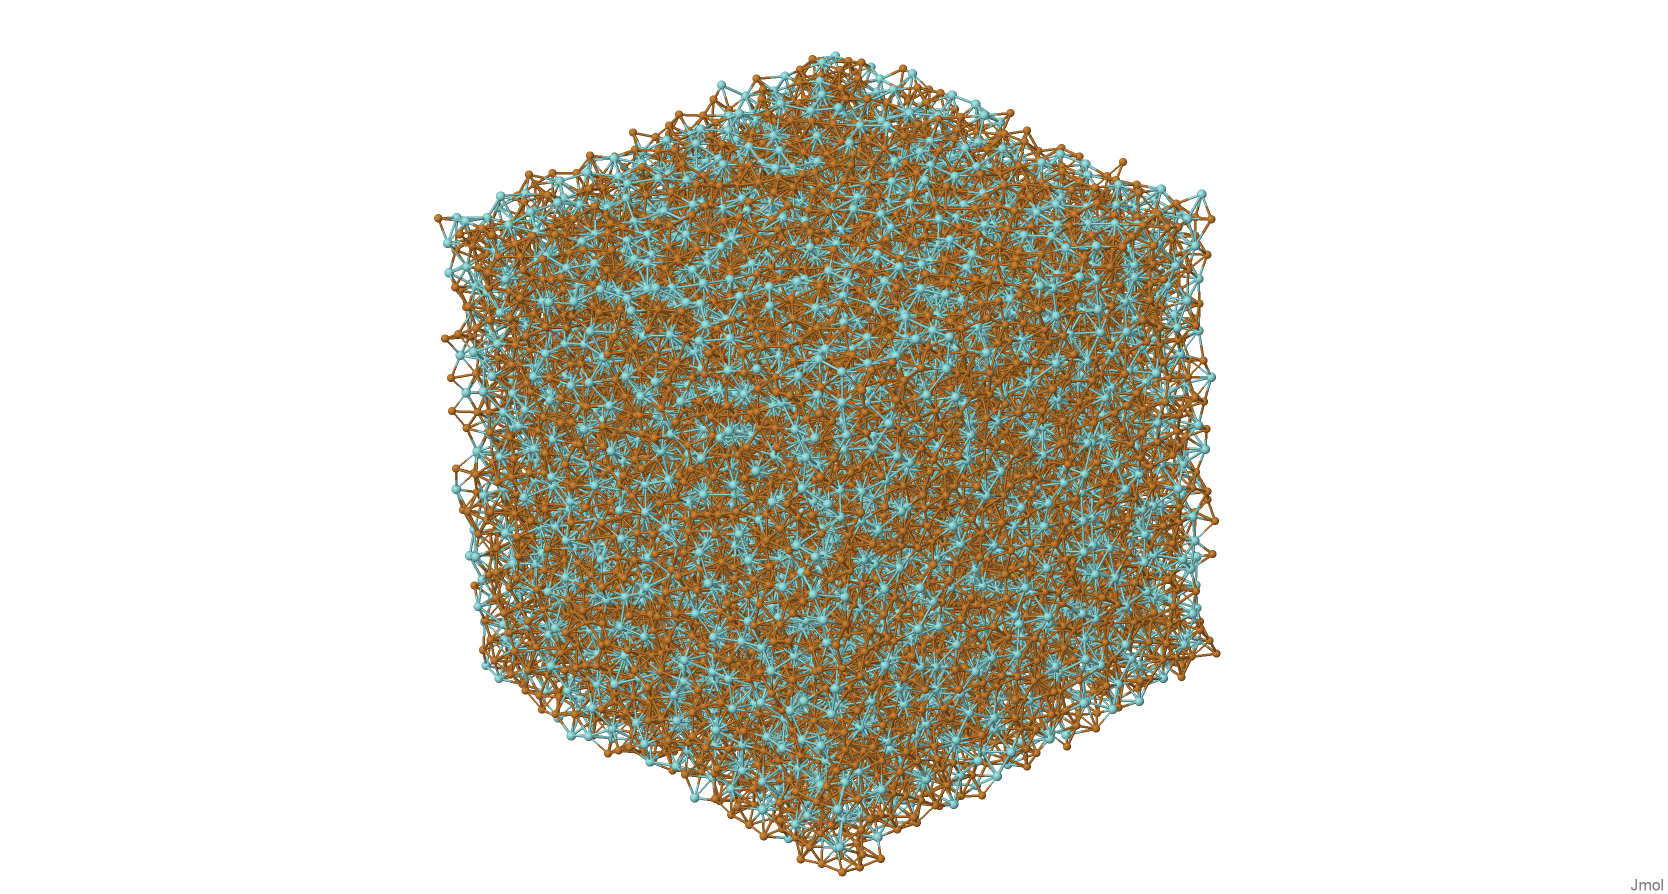
\includegraphics[width=0.99\textwidth]{Cu8640Zr4860}
  \caption{Amorphous structure $\mathrm{Cu}_{8640}\mathrm{Zr}_{4860}$ with $13,500$ atoms.}
\end{center}
\label{fig:Cu8640Zr4860_jmol}
\end{figure}

Experiments with the geometry of amorphous structures of 
$\mathrm{Cu}_{8640}\mathrm{Zr}_{4860}$ (c.f.~fig.~\ref{fig:Cu8640Zr4860_jmol})
show that it is fairly compute intensive to construct $\hat W$.
However, we can observe that the derivation between matrix elements of $W$ and a simple
sphere volumen overlap model is small, c.f.~fig.\ref{fig:truncation_sphere_overlap_vs_distance}.

\begin{figure}[h!]
\begin{center}
  \includegraphics[width=0.6\textwidth]{truncation_sphere_overlap_vs_distance_new}
  \caption{Model vs data:
  For atom pair distances $d_{aa'}$ larger than $2R\um{trc} = 31.9\,\AA$ the overlap vanishes.
  The count of how many atoms are in both truncation zones coincides well with the sphere volume model.
  The three colors indicate different excerpts from the data sets.
  }
\end{center}
\label{fig:truncation_sphere_overlap_vs_distance}
\end{figure}

\subsection{Sphere volume overlap model}

Assume two spheres of equal radius $R\um{trc}$ whose centers are separated by $d \geq 0$.
For $d > 2 R\um{trc}$ we encounter a vanishing overlap.
For $0 \leq d \leq 2 R\um{trc}$ we can find the model for the overlap $M$ from the lense-shaped body of rotation that
originates from the intersection of two spheres.
The sphere surface is described by $\sqrt{R\um{trc}^2 - x^2}$.
Now,
\begin{align*}
  M &= 2 \pi \int\limits_{\frac 12 d}^{R\um{trc}} \mathrm d x \left( \sqrt{ R\um{trc}^2 - x^2 } \right)^2 \\
    &= 2 \pi \left( \frac 23 R\um{trc}^3 - \frac d2 R\um{trc}^2 + \frac{d^3}{24} \right) \\
    &= \frac{4\pi}{3} \left( R\um{trc}^3 - \frac{3d}{4} R\um{trc}^2 + \frac{d^3}{16} \right) \\
    &= \frac{4\pi}{3} \left( \frac d2 - R\um{trc} \right)^2 \left(\frac d4 + R\um{trc} \right) \\
\end{align*}
Obviously, the function assumes the volumen of one sphere $\frac{4\pi}{3} R\um{trc}^3$ for $d=0$
and connects to the vanishing overlap at $d=2R\um{trc}$ with zero value and derivative 
due to the second power at the linear term $(d/2 - R\um{trc})$.

\begin{figure}[h!]
\begin{center}
  \includegraphics[width=0.6\textwidth]{sphere_volume_overlap_model}
  \caption{Model formula for the overlap of two spheres of unit radius. 
  For a distance $d$ between their centers, the overlap is given by $(d/2 - 1)^2 (d/4 + 1)$.}
\end{center}
\label{fig:sphere_volume_overlap_model}
\end{figure}

\section{Task}

\subsection{Preparations}

In the sources, the generation of the boolean table $Z_{aa'}$
has been implemented. For this, first the pair distance table $d_{aa'}$ is constructed.
Here, a $N_a^2$-scaling ansatz has been taken for simplicity.
This becomes a waste of computing time as we are only interested in atom pair distances
which are smaller than $R\um{trc}$.
If we directly determine $W_{aa'}$ via the sphere volume overlap formula, 
we can omit the computation of $\hat Z$.
However, all atom pair distances must be smaller than $2R\um{trc}$.

The linear scaling ansatz is to construct boxes with edge lengths of at least $2R\um{trc}$.
For each atom, we add the atom to a member list of the box it lies in.
Now we only need to compute atom pairs for which the atom partners are in the same or 
in one of the $26$ direct neighbor boxes.

Even better than boxes would be to use dodecahedra, 
i.e.~an fcc geometry as there would only be $12$ neighbor dodecahedra.

\subsection{Optimization}

We have to maximize the aforementioned overlap on each \MPIrank{}
under the additional constraint of balancing the work among all \MPIrank{}s.
Fortunately, for systems that are filled relatively homogeneously with atoms,
this will leads to compact and convex formations of atoms belonging to the same \MPIrank{}.
Hence, this approach also minimizes the required MPI communication volumes
(and number of communication partners)
which are necessary during the setup of the block-rows of $\hat A$.

\section{Conclusion}

We introduce the problem of assigning atoms to \MPIrank{}s
such that in a KKRnano calculation, 
the best floating-point efficiency of the tfQMR solver is maximized, and
memory consumtion and MPI communication are minimized.

% -- optional
%\section*{Acknowledgments}

\bibliographystyle{plain}
\begin{thebibliography}{10}
\bibitem{zeller_towards_2008} Zeller, Rudolf.;
   \textit{Towards a linear-scaling algorithm for electronic structure calculations with the tight-binding Korringa-Kohn-Rostoker {Green} function method};
    Journal of Physics: Condensed Matter \textbf{20} (2012) 294215;
    [DOI: 10.1088/0953-8984/20/29/294215]
\bibitem{kkrnano:thiess_massively_2012} Thiess, A. and Zeller, R. and Bolten, M. and Dederichs, P. H. and Bl{\"u}gel, S.;
   \textit{Massively parallel density functional calculations for thousands of atoms: {KKRnano}};
    Physical Review B \textbf{85} (2012) 235103;
    [DOI: 10.1103/PhysRevB.85.235103]
\end{thebibliography}

\end{document}


